\documentclass[a4paper,12pt]{article}

\usepackage[utf8]{inputenc}
\usepackage[russian]{babel}
\usepackage{amsmath} 
\usepackage{listings} 
\usepackage{graphicx} 
\usepackage{hyperref} 
\usepackage{xcolor}  

\definecolor{myblue}{rgb}{0.13, 0.13, 1.0}
\definecolor{myred}{rgb}{0.9, 0.1, 0.1}
\definecolor{mygreen}{rgb}{0, 0.5, 0}

\lstset{
    language=Python,
    basicstyle=\ttfamily\small,
    keywordstyle=\color{myblue},
    stringstyle=\color{myred},
    commentstyle=\color{mygreen},
    morekeywords={eval, input, print},
    breaklines=true,
    showstringspaces=false
}



\begin{document}

\begin{titlepage}
    \begin{center}
        \textbf{Министерство науки и высшего образования Российской Федерации}\\[0.5cm]
        
        \textbf{Федеральное государственное автономное образовательное учреждение высшего образования}\\
        \textbf{«Национальный исследовательский университет ИТМО»}

        \begin{figure}[h!]
            \centering
            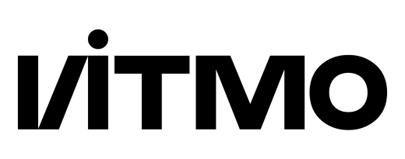
\includegraphics[width=0.7\textwidth]{image.png}
        \end{figure}
        
        \textbf{\large Факультет информационных технологий и программирования}\\[1cm]
        
        \textbf{ Лабораторная работа №3}\\[0.5cm]
        \textbf{ Работа с LaTeX}\\[4cm]
        
        Выполнил студент группы № M3113\\
        Пахомов Глеб Владимирович\\[3cm]
        
        Проверил: \\
        Хасан Карим Асадович / Жуйков Артём Сергеевич\\[2cm]
        
        Санкт-Петербург\\
        2024
    \end{center}
\end{titlepage}

\tableofcontents
\newpage

\section{Общее описание библиотеки}
Библиотека \texttt{geometric\_lib} предназначена для вычисления площадей и периметров различных геометрических фигур, таких как круг, квадрат и треугольник. Программа использует модули Python для вычисления математических формул.

\section{Описание файлов}

\subsection{Файл calculate.py}
\subsubsection{Исходный код}
\begin{lstlisting}
import circle
import square

figs = ['circle', 'square']
funcs = ['perimeter', 'area']
sizes = {}

def calc(fig, func, size):
    assert fig in figs
    assert func in funcs

    result = eval(f'{fig}.{func}(*{size})')
    print(f'{func} of {fig} is {result}')

if __name__ == "__main__":
    func = ''
    fig = ''
    size = list()

    while fig not in figs:
        fig = input(f"Enter figure name, avaliable are {figs}:\n")
    
    while func not in funcs:
        func = input(f"Enter function name, avaliable are {funcs}:\n")
    
    while len(size) != sizes.get(f"{func}-{fig}", 1):
        size = list(map(int, input("Input figure sizes separated by space, 1 for circle and square\n").split(' ')))
    
    calc(fig, func, size)
\end{lstlisting}

\subsubsection{Описание логики}
Скрипт \texttt{calculate.py} позволяет пользователю выбирать фигуру и тип вычислений (площадь или периметр), а затем вводить необходимые параметры для выполнения вычислений.

\subsection{Файл square.py}
\subsubsection{Исходный код}
\begin{lstlisting}
def area(a):
    return a * a

def perimeter(a):
    return 4 * a
\end{lstlisting}

\subsubsection{Описание логики}
Функции для квадрата:
\begin{itemize}
    \item \texttt{area(a)} — вычисляет площадь квадрата по формуле $a^2$.
    \item \texttt{perimeter(a)} — вычисляет периметр квадрата по формуле $4 \cdot a$.
\end{itemize}

\subsection{Файл triangle.py}
\subsubsection{Исходный код}
\begin{lstlisting}
def area(a, b, c):
    return (a + b + c) / 2

def perimeter(a, b, c):
    return a + b + c
\end{lstlisting}

\subsubsection{Описание логики}
Функции для треугольника:
\begin{itemize}
    \item \texttt{area(a, b, c)} — вычисляет площадь треугольника через полупериметр $p = \frac{a + b + c}{2}$.
    \item \texttt{perimeter(a, b, c)} — вычисляет периметр треугольника как сумму сторон $a + b + c$.
\end{itemize}

\subsection{Файл circle.py}
\subsubsection{Исходный код}
\begin{lstlisting}
import math

def area(r):
    return math.pi * r * r

def perimeter(r):
    return 2 * math.pi * r
\end{lstlisting}

\subsubsection{Описание логики}
Функции для круга:
\begin{itemize}
    \item \texttt{area(r)} — вычисляет площадь круга по формуле $S = \pi r^2$.
    \item \texttt{perimeter(r)} — вычисляет периметр круга по формуле $P = 2 \pi r$.
\end{itemize}

\section{Формулы}

\subsection{Площадь}
\begin{itemize}
    \item Круг: $S = \pi r^2$
    \item Квадрат: $S = a^2$
    \item Треугольник: $S = \sqrt{p \cdot (p - a) \cdot (p - b) \cdot (p - c)}$, где $p = \frac{a + b + c}{2}$ — полупериметр
\end{itemize}

\subsection{Периметр}
\begin{itemize}
    \item Круг: $P = 2 \pi r$
    \item Квадрат: $P = 4a$
    \item Треугольник: $P = a + b + c$
\end{itemize}

\section{Заключение}
Библиотека \texttt{geometric\_lib} предоставляет простой и удобный интерфейс для вычисления базовых геометрических характеристик фигур: площади и периметра. Программа поддерживает ввод данных от пользователя и визуализирует формулы для вычислений.

\section{Ссылки}
\begin{itemize}
    \item Проект на GitHub: \href{https://github.com/Cpp-Gleb/geometric_lib/}{geometric\_lib}
    \item Ссылка на Overleaf: \href{https://ru.overleaf.com/read/nfdxcjbzttsg#0f783f}{Overleaf}
\end{itemize}

\end{document}
